\section{Posicionando semillas}

Una forma r\'apida y sencilla de validar el correcto funcionamiento del algoritmo
es, partiendo de una parcelaci\'on ya existente, pintar cada semilla resultante 
del color de la parcela de la cual se comenz\'o. Las semillas generadas deber\'ian
estar a la distancia deseada de la corteza, compartiendo el color de alguna de
las parcelas mas cercanas.\\

La Figura \ref{fig:semillas} muestra donde fueron posicionadas las semillas en
la materia blanca del hemisferio izquierdo. El color de cada semilla representa
el \'area del cual proviene.

\begin{figure}[h!]
   \centering
    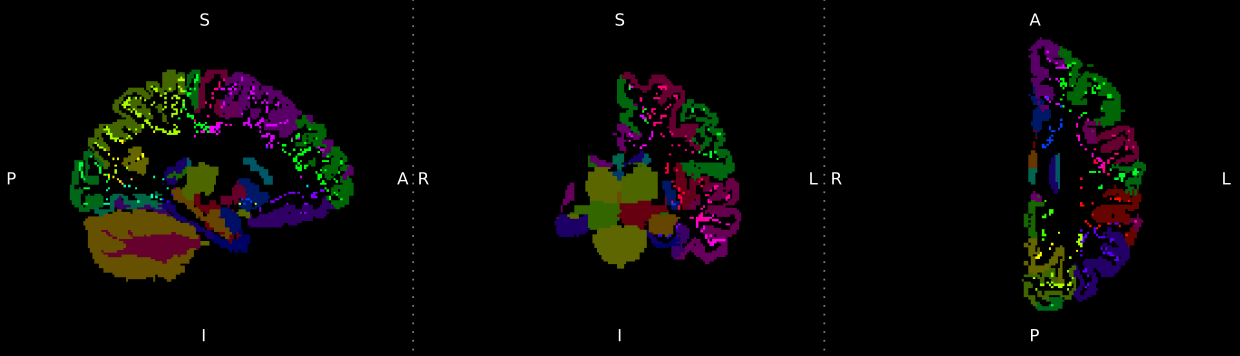
\includegraphics[width=\textwidth]{img/painted_seeds.png}
    \caption{Semillas en el hemisferio izquierdo. }
    \label{fig:semillas}
\end{figure}

